\documentclass[crop]{standalone}

\usepackage{mhocolorpalettesthlmnord}
\usepackage{mhofonts}
\usepackage{mhomacros}
\usepackage{mhotikz}
\begin{document}

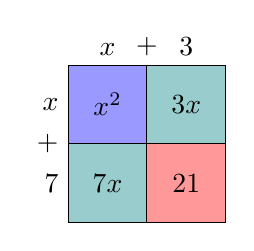
\begin{tikzpicture}
\draw[fill=Teal!40] (0,1) rectangle (1,2);
\draw[fill=Red!40] (1,1) rectangle (2,2);
\draw[fill=Blue!40] (0,2) rectangle (1,3);
\draw[fill=Teal!40] (1,2) rectangle (2,3);

% Summands of the Factors
\draw (0,2.5) node[left]{\(x\)};
\draw (0,2) node[left]{\(+\)};
\draw (0,1.5) node[left]{\(\oneg 7\)};

\draw (0.5,3) node[above]{\(x\)};
\draw (1,3) node[above]{\(+\)};
\draw (1.5,3) node[above]{\(3\)};

% Row 1
\draw (0.5,2.5) node{\(x^2\)};
\draw (1.5,2.5) node{\(3x\)};

% Row 2
\draw (0.5,1.5) node{\(\oneg 7x\)};
\draw (1.5,1.5) node{\(\oneg 21\)};

\end{tikzpicture}


\end{document}